\section{Tensor de Similaridade em Espaços de Hilbert com Núcleo Reprodutor}\label{sec:tensor_rkhs}

A Seção \ref{sec:rkhs} estabeleceu os fundamentos dos RKHS, demonstrando que todo \textit{kernel} simétrico e positivamente definido determina um único RKHS, e que o produto de \textit{kernels} positivamente definidos é também positivamente definido. Esta seção desenvolve, sobre esses fundamentos, a base matemática do método proposto, isto é, o tensor de similaridade construído via produto tensorial de RKHS, e os seus resultados, junto com os das Seções \ref{sec:kernel_pipeline} e \ref{sec:representation_geometry}, constituem a principal contribuição deste trabalho. A construção é apresentada em quatro etapas: o produto tensorial de espaços de Hilbert, o tensor de similaridade como núcleo reprodutor do produto tensorial, a estrutura métrica via curvas de nível, e o complemento ortogonal de RKHS. Cada etapa é fundamentada por demonstrações dos resultados centrais, sem referência a aplicações específicas. Observe que nenhum desses resultados depende de quais são as $d$ fontes ou de quais \textit{kernels} são utilizados, sendo exigido apenas que cada $k_l$ seja positivamente definido. A forma como essa teoria é aplicada sobre uma amostra finita é apresentada na Seção \ref{sec:kernel_pipeline}, enquanto a instanciação utilizada nos experimentos é apresentada na Seção \ref{sec:metodologia}.

\subsection{Produto Tensorial de Espaços de Hilbert}

A questão central que motiva esta construção é a seguinte: dados $d$ espaços de Hilbert independentes, cada um codificando uma forma de similaridade sobre um mesmo conjunto $\mathcal{X}$, como construir um espaço único que codifique todas as similaridades simultaneamente, de tal modo que a estrutura de produto interno seja preservada? A resposta é fornecida pelo produto tensorial.

\textbf{Tensor Elementar:} Sejam $\mathcal{H}_1, \mathcal{H}_2, \dots, \mathcal{H}_d$ espaços de Hilbert. Um tensor elementar é um objeto da forma $f_1 \otimes f_2 \otimes \cdots \otimes f_d$, com $f_l \in \mathcal{H}_l$ para cada $l \in \{1, \dots, d\}$. O símbolo $\otimes$ é multilinear, isto é, para quaisquer escalares $\alpha, \beta \in \mathbb{R}$ e quaisquer $f_l, g_l \in \mathcal{H}_l$:

\begin{equation}\label{eq:tensor_multilinear}
    f_1 \otimes \cdots \otimes (\alpha f_l + \beta g_l) \otimes \cdots \otimes f_d = \alpha (f_1 \otimes \cdots \otimes f_l \otimes \cdots \otimes f_d) + \beta (f_1 \otimes \cdots \otimes g_l \otimes \cdots \otimes f_d).
\end{equation}

O tensor elementar não é uma soma nem um produto ordinário de funções. Ele é um objeto que vive em um espaço novo e representa uma interação multilinear entre os fatores $f_1, \dots, f_d$. Sua decomposição em fatores não é única, pois diferentes reescalonamentos podem representar o mesmo tensor, mas a estrutura conjunta definida por esses fatores é preservada no produto tensorial.

\textbf{Produto Tensorial de Espaços de Hilbert:} Considere o espaço vetorial das combinações lineares finitas de tensores elementares,

\begin{equation}\label{eq:tensor_space}
    \mathcal{T}_0 = \left\{ \sum_{m=1}^{N} c_m \, f_1^{(m)} \otimes f_2^{(m)} \otimes \cdots \otimes f_d^{(m)} \, : \, N \in \mathbb{N}, \, c_m \in \mathbb{R}, \, f_l^{(m)} \in \mathcal{H}_l \right\},
\end{equation}

\noindent modulado pelas relações de multilinearidade \eqref{eq:tensor_multilinear}. Sobre $\mathcal{T}_0$ define-se uma forma bilinear simétrica

\begin{equation}\label{eq:tensor_inner}
    \left\langle \bigotimes_{l=1}^{d} f_l, \; \bigotimes_{l=1}^{d} g_l \right\rangle = \prod_{l=1}^{d} \langle f_l, g_l \rangle_{\mathcal{H}_l},
\end{equation}

\noindent estendida por bilinearidade às combinações lineares finitas. O produto tensorial algébrico $\mathcal{T}_0 = \bigotimes_{l=1}^{d} \mathcal{H}_l$ é então o espaço de Hilbert definido como o completamento com respeito à norma $\|u\| = \sqrt{\langle u,u \rangle}$.

A consequência crucial expressa por \eqref{eq:tensor_inner} é que o produto interno no espaço tensorial se fatora: a similaridade entre dois tensores elementares é o produto das similaridades componente a componente. Esta propriedade é a base de todos os resultados subsequentes desta seção.

\begin{proposition}[Produto interno bem definido e positivo definido]\label{prop:inner_well_defined}
A forma bilinear definida em \eqref{eq:tensor_inner} estende-se por bilinearidade a um produto interno bem definido, simétrico e positivo definido sobre o produto tensorial algébrico $\mathcal{T}_0 = \bigotimes_{l=1}^{d} \mathcal{H}_l$.
\end{proposition}

\begin{proof}
A bilinearidade e a simetria decorrem diretamente das propriedades dos produtos internos em cada espaço componente $\mathcal{H}_l$. Para verificar a positividade, considere $u = \sum_{m} c_m \bigotimes_{l} f_l^{(m)} \in \mathcal{T}_0$. Pela bilinearidade, $\langle u,u\rangle = \sum_{m} \sum_{n} c_m c_n \prod_{l} \left\langle f_l^{(m)},f_l^{(n)} \right\rangle_{\mathcal{H}_l}$. Para cada $l$, seja $E_l = \operatorname{span} \left\{f_l^{(1)},\dots,f_l^{(N)} \right\} \subseteq \mathcal{H}_l$.

\noindent Como $E_l$ é finito-dimensional, escolha uma base ortonormal $\{e_{l,1},\dots,e_{l,r_l}\}$ de $E_l$. Então $u$ pode ser escrito de maneira única na forma

\begin{equation*}
    u = \sum_{i_1=1}^{r_1} \cdots \sum_{i_d=1}^{r_d} a_{i_1,\dots,i_d}\, e_{1,i_1}\otimes\cdots\otimes e_{d,i_d}.
\end{equation*}

\noindent Pela definição do produto interno tensorial e pela ortonormalidade das bases, os tensores $e_{1,i_1}\otimes\cdots\otimes e_{d,i_d}$ são ortonormais. Consequentemente,

\begin{equation*}
    \langle u,u\rangle = \sum_{i_1=1}^{r_1} \cdots \sum_{i_d=1}^{r_d} |a_{i_1,\dots,i_d}|^2 \geq 0.
\end{equation*}

\noindent Além disso, $\langle u,u\rangle=0$ se e somente se todos os coeficientes $a_{i_1,\dots,i_d}$ são nulos, isto é, se e somente se $u=0$. Portanto, a forma é positiva definida e constitui um produto interno sobre $\mathcal{T}_0$.
\end{proof}

\begin{remark}[Dimensionalidade do produto tensorial]\label{rem:tensor_dim}
Quando cada $\mathcal{H}_l$ tem dimensão finita $D_l$, o produto tensorial $\bigotimes_{l=1}^{d} \mathcal{H}_l$ tem dimensão $\prod_{l=1}^{d} D_l$. As dimensões se multiplicam, não se somam. Em termos geométricos, isso reflete o fato de que um par de bases $\{e_i^{(1)}\}$ e $\{e_j^{(2)}\}$ de dois espaços $\mathcal{H}_1$ e $\mathcal{H}_2$ gera uma base $\{e_i^{(1)} \otimes e_j^{(2)}\}$ de $\mathcal{H}_1 \otimes \mathcal{H}_2$ cuja cardinalidade é $D_1 \cdot D_2$. Cada par de direções de cada espaço componente gera uma direção independente no espaço produto, conforme ilustrado na Figura \ref{fig:tensor_product}.
\end{remark}

\begin{figure}[htbp]
    \centering
    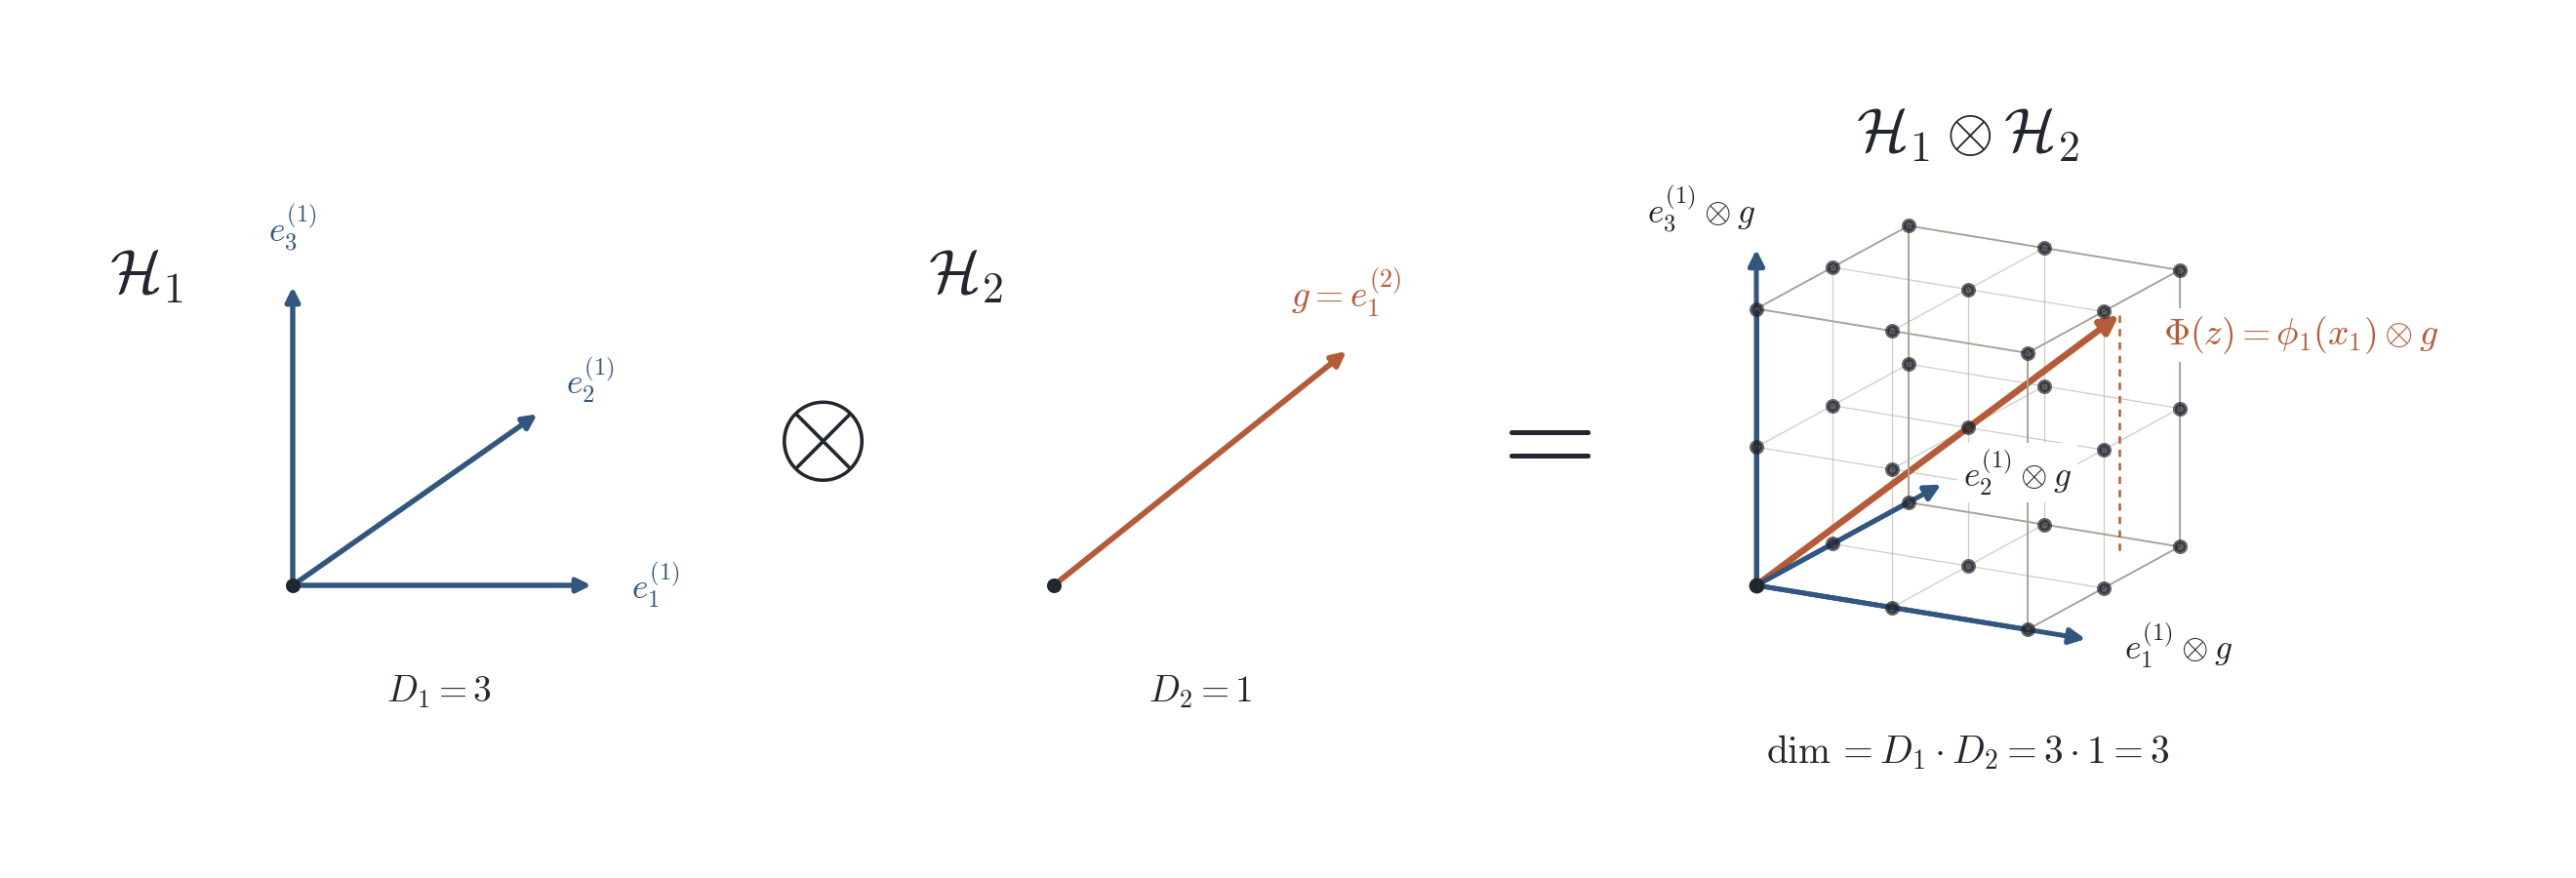
\includegraphics[width=\textwidth]{img/tensor_product_draft}
    \caption{Ilustração do produto tensorial $\mathcal{H}_1 \otimes \mathcal{H}_2$. Cada vetor da base $\{e_i^{(1)}\}$ de $\mathcal{H}_1$, com $D_1 = 3$, combinado ao vetor $g = e_1^{(2)}$ de $\mathcal{H}_2$, com $D_2 = 1$, gera uma direção $e_i^{(1)} \otimes g$ do espaço produto, cuja dimensão é $D_1 \cdot D_2 = 3$. O tensor de similaridade $\Phi(z) = \phi_1(x_1) \otimes g$ é um elemento desse espaço.}
    \label{fig:tensor_product}
\end{figure}

\subsection{Tensor de Similaridade sobre o Domínio Produto}
 
O objeto de análise deste trabalho não é um ponto de um domínio único, mas uma \emph{tupla} de fontes de informação. Sejam $\mathcal{X}_1, \dots, \mathcal{X}_d$ os domínios das $d$ fontes, cada um munido de um \textit{kernel} positivamente definido $k_l$, com RKHS $\mathcal{H}_{k_l}$ e mapa de características canônico $\phi_l(x_l) = k_l(\cdot, x_l)$. A unidade analisada vive no domínio produto
\begin{equation}\label{eq:product_domain}
    \mathcal{Z} = \mathcal{X}_1 \times \mathcal{X}_2 \times \cdots \times \mathcal{X}_d.
\end{equation}
 
\begin{definition}[Tensor de similaridade]\label{def:tensor_sim}
Para uma observação $z = (x_1, \dots, x_d) \in \mathcal{Z}$, o \emph{tensor de similaridade} é a representação tensorial
\begin{equation}\label{eq:tensor_sim_def}
    \Phi(z) = \phi_1(x_1) \otimes \cdots \otimes \phi_d(x_d) = \bigotimes_{l=1}^{d} \phi_l(x_l) \; \in \; \bigotimes_{l=1}^{d} \mathcal{H}_{k_l},
\end{equation}
cujo produto interno é dado pelo \textit{kernel} produto sobre $\mathcal{Z}$,
\begin{equation}\label{eq:tensor_sim_inner}
    K(z, z') = \langle \Phi(z), \Phi(z') \rangle = \prod_{l=1}^{d} \langle \phi_l(x_l), \phi_l(x_l') \rangle_{\mathcal{H}_{k_l}} = \prod_{l=1}^{d} k_l(x_l, x_l'),
\end{equation}
\noindent com $z = (x_1,\dots,x_d)$ e $z' = (x_1',\dots,x_d')$.

\end{definition}
 
\textbf{O tensor é implícito, a Gram o representa.} O tensor de similaridade $\Phi(z)$ é um objeto implícito, em geral de dimensão elevada ($\prod_l D_l$), que não precisa ser exibido explicitamente para que a estrutura de $\mathcal{H}_K$ seja acessível. Toda a informação relevante sobre um conjunto finito $\{z_1, \dots, z_n\}$, com $z_i = (x_{i1}, \dots, x_{id})$, reside nos produtos internos $\langle \Phi(z_i), \Phi(z_j)\rangle$, reunidos na \emph{matriz de Gram} $\mathbf{G}$. Por \eqref{eq:tensor_sim_inner}, essa matriz é o produto de Hadamard das Gram componentes:
\begin{equation}\label{eq:tensor_sim_gram}
    G_{ij} = \prod_{l=1}^{d} k_l(x_{il}, x_{jl}), \hspace{0.2cm} \text{isto é,} \hspace{0.2cm} \mathbf{G} = \mathbf{K}_1 \circ \mathbf{K}_2 \circ \cdots \circ \mathbf{K}_d, \quad (\mathbf{K}_l)_{ij} = k_l(x_{il}, x_{jl}).
\end{equation}
A matriz $\mathbf{G}$ é, assim, a realização finita do tensor de similaridade sobre a amostra: os objetos que caracterizam $\mathcal{H}_K$ se exprimem por meio dela, e não pelos tensores. A Figura \ref{fig:gram_hadamard} ilustra essa composição para $d = 3$ componentes.

\begin{figure}[htbp]
    \centering
    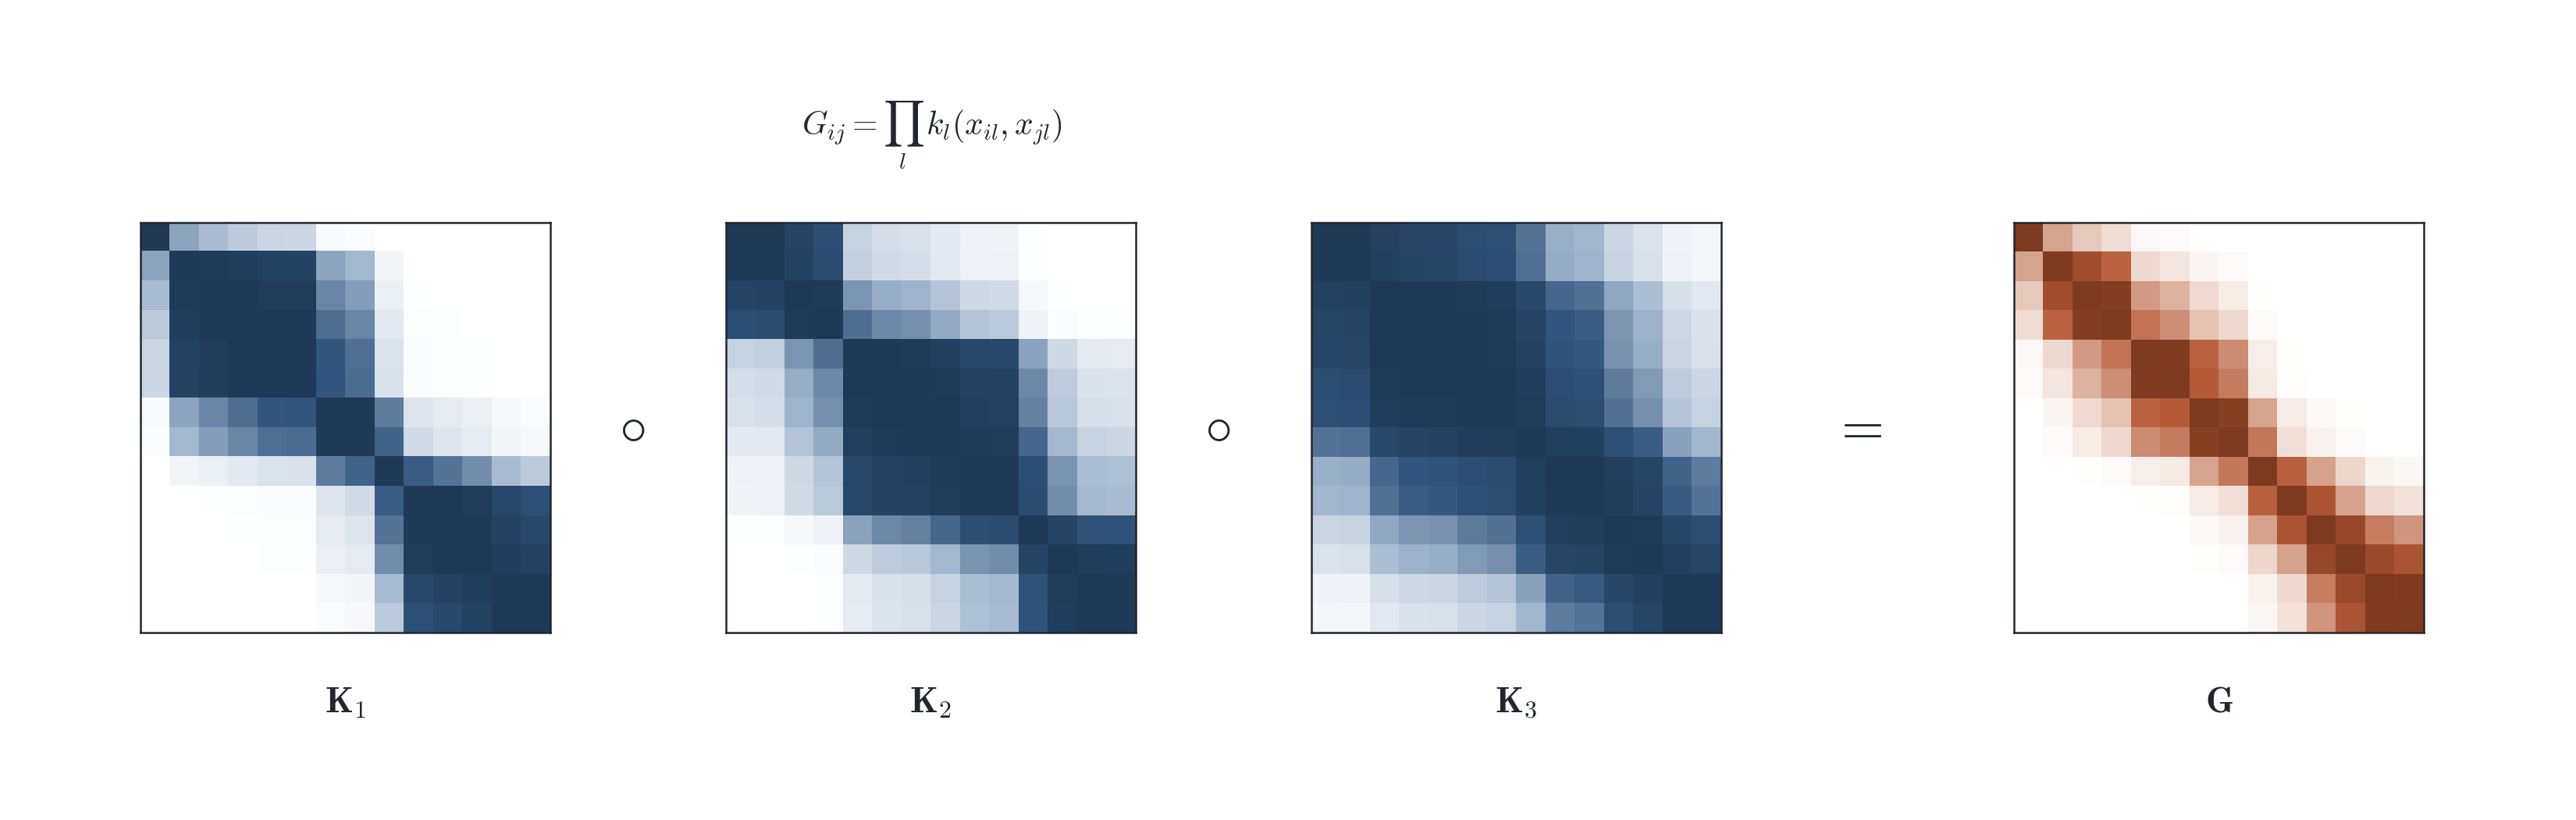
\includegraphics[width=\textwidth]{img/gram_hadamard_draft.png}
    \caption{Ilustração da matriz de Gram do tensor de similaridade como produto de Hadamard das matrizes de Gram componentes, $G_{ij} = \prod_l k_l(x_{il}, x_{jl})$. Veja que a matriz $\mathbf{G}$ só apresenta valores altos nas regiões em que as três componentes $\mathbf{K}_1$, $\mathbf{K}_2$ e $\mathbf{K}_3$ são simultaneamente altas, o que reflete o critério de similaridade conjunta do Comentário \ref{rem:joint_similarity}.}
    \label{fig:gram_hadamard}
\end{figure}
 
A escolha de trabalhar sobre o domínio produto $\mathcal{Z}$, e não sobre um domínio único com os fatores avaliados no mesmo ponto, é o que garante a forma limpa do teorema a seguir: como cada componente $x_l$ varia independentemente em $\mathcal{X}_l$, o tensor de similaridade percorre \emph{todos} os tensores elementares, e não apenas os diagonais.

 
\begin{theorem}[Realização do tensor de similaridade em RKHS]\label{thm:tensor_similarity}
Sejam $\mathcal{H}_{k_1}, \dots, \mathcal{H}_{k_d}$ RKHS com núcleos $k_1, \dots, k_d$ sobre domínios $\mathcal{X}_1, \dots, \mathcal{X}_d$, e seja $K$ o \textit{kernel} produto sobre $\mathcal{Z} = \prod_l \mathcal{X}_l$ definido por
\begin{equation}\label{eq:K_thm}
    K(z, z') = \prod_{l=1}^{d} k_l(x_l, x_l'), \qquad z = (x_1,\dots,x_d), \; z' = (x_1',\dots,x_d').
\end{equation}
Então $K$ é positivamente definido, e seu RKHS $\mathcal{H}_K$ é canonicamente isométrico ao produto tensorial \emph{completo},
\begin{equation}\label{eq:full_iso}
    \mathcal{H}_K \;\cong\; \bigotimes_{l=1}^{d} \mathcal{H}_{k_l},
\end{equation}
sob a identificação $\Phi(z) \mapsto K(\cdot, z)$.
\end{theorem}
 
\begin{proof}
A demonstração tem três passos.
 
\noindent \textit{(i) $K$ é positivamente definido.} Pela Equação \eqref{eq:kernel_prod} (Seção \ref{sec:rkhs}), o produto de \textit{kernels} positivamente definidos é positivamente definido, pelo Teorema de \cite{Aronszajn1950}, $K$ determina um único RKHS, denotado $\mathcal{H}_K$.
 
\noindent \textit{(ii) $\Phi$ preserva o produto interno.} Cada fator $\phi_l(x_l) = k_l(\cdot, x_l)$ pertence a $\mathcal{H}_{k_l}$, de modo que $\Phi(z)$ é um tensor elementar legítimo. Por \eqref{eq:tensor_inner} e pela propriedade reprodutora em cada fator,
\begin{equation*}
    \langle \Phi(z), \Phi(z') \rangle_{\bigotimes \mathcal{H}_{k_l}}
\end{equation*}
\begin{equation*}
    = \prod_{l=1}^{d} \langle k_l(\cdot, x_l), k_l(\cdot, x_l') \rangle_{\mathcal{H}_{k_l}}
\end{equation*}
\begin{equation*}
    = \prod_{l=1}^{d} k_l(x_l, x_l') = K(z, z') = \langle K(\cdot, z), K(\cdot, z') \rangle_{\mathcal{H}_K}.
\end{equation*}
Logo o mapa $\Phi(z) \mapsto K(\cdot, z)$, estendido por linearidade ao span dos tensores de similaridade, preserva o produto interno, é uma isometria linear.
 
\noindent \textit{(iii) Densidade nos dois lados.} Por definição de RKHS, o span de $\{K(\cdot, z) : z \in \mathcal{Z}\}$ é denso em $\mathcal{H}_K$. Reciprocamente, como cada $x_l$ varia \emph{independentemente} em $\mathcal{X}_l$ e o span de $\{k_l(\cdot, x_l)\}$ é denso em $\mathcal{H}_{k_l}$, a multilinearidade e a continuidade de $\otimes$ garantem que o span de $\{\Phi(z)\}$ seja denso em $\bigotimes_l \mathcal{H}_{k_l}$. Uma isometria definida num subespaço denso estende-se de modo único, por continuidade, a uma isometria \emph{sobrejetora} entre os fechos, obtém-se assim o isomorfismo \eqref{eq:full_iso}. A variação independente dos $x_l$ é o passo decisivo: sem ela, o span conteria apenas tensores diagonais e não seria denso (Comentário \ref{rem:diagonal_case}).
\end{proof}
 
\begin{remark}[Caso diagonal e suporte dos dados]\label{rem:diagonal_case}
A hipótese decisiva do Teorema \ref{thm:tensor_similarity} é a variação independente das componentes. Se, em vez disso, as $d$ fontes forem todas derivadas de um mesmo objeto subjacente $x$, por um mapa de acoplamento $x \mapsto (x_1(x), \dots, x_d(x))$, as observações vivem numa subvariedade acoplada de $\mathcal{Z}$ (o ``caso diagonal''), e o span de $\{\Phi\}$ gera apenas um subespaço \emph{próprio} de $\bigotimes_l \mathcal{H}_{k_l}$. Nesse regime, ainda que o isomorfismo \eqref{eq:full_iso} descreva o objeto no nível do domínio, a dimensão \emph{efetiva} suportada pelas observações satisfaz $\mathrm{rank}(\mathbf{G}) \leq n$, em geral abaixo de $\prod_l D_l$: é uma propriedade do suporte amostral, não do núcleo, e não afeta o teorema nem a forma da Gram $\mathbf{G} = \mathbf{K}_1 \circ \cdots \circ \mathbf{K}_d$.
\end{remark}
 
\begin{corollary}[Forma matricial]\label{cor:hadamard_form}
Sejam $\{z_1, \dots, z_n\} \subset \mathcal{Z}$ um conjunto finito e $\mathbf{K}_l$ a matriz de Gram de $k_l$ nas $l$-ésimas componentes. A matriz de Gram do \textit{kernel} produto é o produto de Hadamard $\mathbf{G} = \mathbf{K}_1 \circ \cdots \circ \mathbf{K}_d$, simétrica e semidefinida positiva.
\end{corollary}
 
\begin{proof}
A entrada $(i,j)$ de $\mathbf{K}_1 \circ \cdots \circ \mathbf{K}_d$ é $\prod_l (\mathbf{K}_l)_{ij} = \prod_l k_l(x_{il}, x_{jl}) = K(z_i, z_j)$. A simetria é preservada pelo produto de Hadamard de matrizes simétricas, e a semidefinição positiva decorre do teorema de Schur \citep{Schur1911, HornJohnson2013}.
\end{proof}
 

\begin{remark}[Critério de similaridade conjunta]\label{rem:joint_similarity}
A forma multiplicativa de \eqref{eq:K_thm} impõe um critério de similaridade \emph{conjunta}: assumindo $k_l \geq 0$ (como em \textit{kernels} normalizados), para que $K(z, z')$ seja grande é necessário que todo $k_l(x_l, x_l')$ seja grande. Um único fator próximo de zero suprime o produto, como pode ser observado na Figura \ref{fig:gram_hadamard}. Isso difere qualitativamente de uma combinação aditiva $\sum_l \alpha_l k_l$, em que um fator dominante poderia mascarar a discordância dos demais. Quando os $k_l$ podem ser negativos, a interpretação exige cuidado, pois cancelamentos de sinal podem produzir $K(z,z')$ pequeno mesmo com fatores individuais não pequenos em módulo.
\end{remark}

\begin{corollary}[Composição recursiva]\label{cor:recursive_composition}
Sejam $\mathcal{H}_{K^{(1)}}, \dots, \mathcal{H}_{K^{(L)}}$ RKHS, cada um já construído como o RKHS de um \textit{kernel} produto via Teorema \ref{thm:tensor_similarity}. Então o RKHS do \textit{kernel} produto $K_{\mathrm{tot}} = \prod_{\ell=1}^{L} K^{(\ell)}$ é canonicamente isométrico a $\bigotimes_{\ell=1}^{L} \mathcal{H}_{K^{(\ell)}}$.
\end{corollary}

\begin{proof}
Aplicação iterada do Teorema \ref{thm:tensor_similarity}, tomando os RKHS $\mathcal{H}_{K^{(\ell)}}$ como espaços componentes.
\end{proof}

A composição em níveis hierárquicos preserva, assim, a estrutura de RKHS: o \textit{kernel} total é o produto dos \textit{kernels} de nível, e o objeto que o realiza é novamente um tensor de similaridade. Essa propriedade permite estender o método descrito na Seção \ref{sec:kernel_pipeline} a níveis hierárquicos, como a composição entre camadas de um modelo construída sobre o produto tensorial entre fontes dentro de cada camada. Entretanto, essa extensão não é explorada na instanciação apresentada na Seção \ref{sec:metodologia}, que analisa cada camada separadamente.

\subsection{Estrutura Métrica via Curvas de Nível}\label{subsec:metric}
 
Estabelecida a realização de $\mathcal{H}_K$, resta dotá-lo de uma estrutura métrica utilizável. A estrutura natural é a distância induzida pela norma de $\mathcal{H}_K$.
 
\textbf{Distância no RKHS.} Seja $\Phi(z) = K(\cdot, z)$ o mapa canônico. A distância entre duas representações é
\begin{equation}\label{eq:rkhs_distance}
    \|\Phi(z) - \Phi(z')\|_{\mathcal{H}_K}^2 = K(z, z) + K(z', z') - 2 K(z, z'),
\end{equation}
que decorre da expansão da norma da diferença e da identificação $\langle \Phi(z), \Phi(z')\rangle_{\mathcal{H}_K} = K(z, z')$. Trata-se de uma medida par a par de natureza global, inteiramente calculável a partir de $\mathbf{G}$: quantifica a similaridade entre dois pontos, mas não exibe, por si só, como a representação varia na vizinhança de uma referência.
 
\textbf{Curvas de nível.} Para explicitar a estrutura local em torno de uma referência $z_0 \in \mathcal{Z}$, define-se a função distância $p(z) = \|\Phi(z) - \Phi(z_0)\|_{\mathcal{H}_K}$ e, para cada raio $r > 0$, o conjunto de nível
\begin{equation}\label{eq:level_curve}
    \Gamma_r(z_0) = \{ z \in \mathcal{Z} : p(z) = r \},
\end{equation}
formado pelos pontos equidistantes de $z_0$ na métrica de $\mathcal{H}_K$. À medida que $r$ cresce, os conjuntos $\Gamma_r(z_0)$ organizam $\mathcal{Z}$ em camadas de equidistância em torno de $z_0$.
 
\begin{proposition}[Propriedades de $p$]\label{prop:dist_props}
A função $p$ satisfaz: \textnormal{(i)} $p(z) \geq 0$, com $p(z) = 0$ se e somente se $K(\cdot, z) = K(\cdot, z_0)$ como funções, \textnormal{(ii)} $p$ é contínua na topologia induzida por $K$ e \textnormal{(iii)} onde $p$ é diferenciável, $\nabla p$ é perpendicular aos conjuntos de nível $\Gamma_r(z_0)$.
\end{proposition}
 
\begin{proof}
(i) decorre de $\|v\| = 0 \iff v = 0$ em espaços de Hilbert. (ii) decorre da continuidade da norma e da avaliação pontual em RKHS \citep{Aronszajn1950}. (iii) é a propriedade clássica de que o gradiente de uma função escalar é perpendicular às superfícies onde ela é constante.
\end{proof}
 
\begin{remark}[Separabilidade de pontos]\label{rem:point_sep}
A implicação $p(z) = 0 \Rightarrow z = z_0$ requer que $K$ separe pontos. Isso é satisfeito, por exemplo, por \textit{kernels} estritamente positivamente definidos. Quando falha, a análise deve ser feita no quociente de $\mathcal{Z}$ pela relação $z \sim z_0 \iff K(\cdot, z) = K(\cdot, z_0)$.
\end{remark}
 
A utilidade dos conjuntos de nível é qualitativa: a rapidez com que $p$ cresce ao redor de $z_0$ indica a estabilidade local da representação. Regiões em que pequenos deslocamentos produzem grande variação de $p$ são regiões sensíveis, e regiões em que $p$ varia pouco são estáveis. Essa informação complementa a distância par a par \eqref{eq:rkhs_distance}, que sozinha não a exibe.
 
\subsection{Subespaço Espectral e Energia Ortogonal}\label{subsec:spectral}
 
A análise da subseção anterior descreve a métrica de $\mathcal{H}_K$. Resta caracterizar como a energia das representações se distribui entre os modos espectrais do núcleo, distinguindo as direções dominantes daquelas excluídas pelo truncamento espectral. Essa caracterização é obtida por meio da decomposição espectral de $K$.
 
\textbf{Decomposição de Mercer.} Seja $\mu$ uma medida finita sobre $\mathcal{Z}$ e seja $T_K : L^2(\mathcal{Z},\mu) \to L^2(\mathcal{Z},\mu)$ o operador integral definido por
\begin{equation}\label{eq:integral_operator}
    (T_K f)(z)
    =
    \int_{\mathcal{Z}}
    K(z,z')\,f(z')\,d\mu(z').
\end{equation}
Se $K$ é contínuo, simétrico e positivamente definido, e $\mathcal{Z}$ é compacto, o teorema de Mercer garante a expansão
\begin{equation}\label{eq:mercer}
    K(z,z')
    =
    \sum_{k=1}^{\infty}
    \lambda_k\,\psi_k(z)\,\psi_k(z'),
    \qquad
    \lambda_1 \geq \lambda_2 \geq \cdots \geq 0,
\end{equation}
em que $\{\psi_k\}$ é um sistema ortonormal de autofunções de $T_K$ em $L^2(\mathcal{Z},\mu)$ \citep{Mercer1909, Aronszajn1950}. Para os autovalores positivos, o conjunto
\begin{equation*}
    \left\{
        \sqrt{\lambda_k}\,\psi_k
    \right\}_{\lambda_k>0}
\end{equation*}
forma uma base ortonormal de $\mathcal{H}_K$. Cada termo da expansão corresponde a um modo espectral independente, e o autovalor $\lambda_k$ quantifica a contribuição global desse modo para a estrutura do operador integral associado ao núcleo.

Empiricamente, quando se dispõe apenas da matriz de Gram
\begin{equation*}
    \mathbf{G}
    =
    V\Lambda V^\top,
\end{equation*}
os autovalores e autovetores de $\mathbf{G}$ fornecem uma aproximação finita da decomposição de Mercer. As colunas de $V$ representam as direções espectrais observadas na amostra, enquanto os elementos diagonais de $\Lambda$ quantificam a contribuição de cada uma dessas direções.
 
\textbf{Subespaço espectral retido.} Retêm-se os $r$ modos de maior autovalor:
\begin{equation}\label{eq:V_r}
    V_r
    =
    \mathrm{span}
    \left(
        \sqrt{\lambda_1}\,\psi_1,
        \dots,
        \sqrt{\lambda_r}\,\psi_r
    \right)
    \subset \mathcal{H}_K,
\end{equation}
em que o número $r$ de modos retidos precisa ser escolhido. Uma primeira regra fixa um limiar $\tau \in (0,1)$ e toma o menor número de modos cuja energia espectral acumulada atinja a proporção $\tau$:
\begin{equation}\label{eq:r_threshold}
    r
    =
    \min
    \left\{
        r' :
        \frac{
            \sum_{k=1}^{r'} \lambda_k
        }{
            \sum_k \lambda_k
        }
        \geq \tau
    \right\}.
\end{equation}
A ponderação por $\lambda_k$ corresponde à convenção utilizada em análise de componentes principais no espaço de características e expressa a proporção da energia espectral total associada aos modos retidos. O valor de $\tau$ controla a granularidade da representação: valores próximos de $1$ preservam um número maior de modos e produzem subespaços mais ricos, enquanto valores menores produzem representações mais compactas e dominadas pelos componentes de maior autovalor.

Uma segunda regra, que não exige a escolha de um limiar, é a razão de participação
\begin{equation}\label{eq:r_participation}
    r
    =
    \operatorname{round}
    \left(
        \frac{
            \left(\sum_k \lambda_k\right)^2
        }{
            \sum_k \lambda_k^2
        }
    \right),
\end{equation}
que vale $m$ para um espectro com $m$ autovalores iguais e $1$ para um núcleo de posto um, de modo que conta os modos efetivamente ativos em vez de fixar uma proporção de energia. Essa é a regra adotada nos experimentos da Seção \ref{sec:metodologia}. Em qualquer das duas regras, o complemento ortogonal $V_r^\perp$ contém as direções de $\mathcal{H}_K$ excluídas pelo truncamento espectral.
 
\begin{proposition}[Decomposição ortogonal]\label{prop:ortho_decomp}
Toda função $u \in \mathcal{H}_K$ admite uma decomposição única
\begin{equation}\label{eq:ortho_decomp}
    u
    =
    P_\parallel u
    +
    P_\perp u,
\end{equation}
com $P_\parallel u \in V_r$ e $P_\perp u \in V_r^\perp$. Além disso, vale a identidade de Pitágoras
\begin{equation}\label{eq:pythagoras}
    \|u\|_{\mathcal{H}_K}^2
    =
    \|P_\parallel u\|_{\mathcal{H}_K}^2
    +
    \|P_\perp u\|_{\mathcal{H}_K}^2.
\end{equation}
\end{proposition}
 
\begin{proof}
Como $V_r$ possui dimensão finita, ele é um subespaço fechado de $\mathcal{H}_K$. O resultado segue diretamente do teorema da projeção aplicado à soma direta ortogonal
\begin{equation*}
    \mathcal{H}_K
    =
    V_r
    \oplus
    V_r^\perp.
\end{equation*}
A identidade de Pitágoras decorre da ortogonalidade
\begin{equation*}
    \left\langle
        P_\parallel u,
        P_\perp u
    \right\rangle_{\mathcal{H}_K}
    =
    0.
\end{equation*}
\end{proof}
 
\textbf{Energia espectral de uma amostra.} Para uma observação $z \in \mathcal{Z}$, considere sua representação canônica
\begin{equation*}
    u_z
    =
    \Phi(z)
    =
    K(\cdot,z)
    \in
    \mathcal{H}_K.
\end{equation*}
Pela expansão de Mercer, essa representação pode ser escrita como
\begin{equation}\label{eq:sample_expansion}
    u_z
    =
    \sum_{k=1}^{\infty}
    \sqrt{\lambda_k}\,\psi_k(z)
    \left(
        \sqrt{\lambda_k}\,\psi_k
    \right).
\end{equation}
Como $\{\sqrt{\lambda_k}\psi_k\}_{\lambda_k>0}$ é uma base ortonormal de $\mathcal{H}_K$, a contribuição energética do $k$-ésimo modo para a representação da amostra $z$ é
\begin{equation}\label{eq:sample_mode_energy}
    E_k(z)
    =
    \lambda_k\,\psi_k(z)^2.
\end{equation}
A energia total induzida pela amostra é, portanto,
\begin{equation}\label{eq:sample_total_energy}
    E_{\mathrm{total}}(z)
    =
    \|u_z\|_{\mathcal{H}_K}^2
    =
    K(z,z)
    =
    \sum_{k=1}^{\infty}
    \lambda_k\,\psi_k(z)^2.
\end{equation}
Assim, a energia da amostra contida no subespaço espectral retido é
\begin{equation}\label{eq:sample_retained_energy}
    E_\parallel(z)
    =
    \|P_\parallel u_z\|_{\mathcal{H}_K}^2
    =
    \sum_{k=1}^{r}
    \lambda_k\,\psi_k(z)^2,
\end{equation}
enquanto a energia associada ao complemento ortogonal é
\begin{equation}\label{eq:sample_orthogonal_energy}
    E_\perp(z)
    =
    \|P_\perp u_z\|_{\mathcal{H}_K}^2
    =
    \sum_{k>r}
    \lambda_k\,\psi_k(z)^2.
\end{equation}
Pela identidade de Pitágoras,
\begin{equation*}
    E_{\mathrm{total}}(z)
    =
    E_\parallel(z)
    +
    E_\perp(z).
\end{equation*}
 
\textbf{Razão de energia ortogonal.} Para uma observação $z$ cuja representação possui norma não nula, define-se
\begin{equation}\label{eq:e_ratio}
    E_{\mathrm{ratio}}(z)
    =
    \frac{
        E_\perp(z)
    }{
        E_{\mathrm{total}}(z)
    }
    =
    \frac{
        \|P_\perp u_z\|_{\mathcal{H}_K}^2
    }{
        \|u_z\|_{\mathcal{H}_K}^2
    }
    =
    \frac{
        \sum_{k>r}
        \lambda_k\,\psi_k(z)^2
    }{
        \sum_k
        \lambda_k\,\psi_k(z)^2
    }
    \in [0,1].
\end{equation}
Vale $E_{\mathrm{ratio}}(z)=0$ quando a representação da amostra pertence integralmente ao subespaço retido $V_r$, e $E_{\mathrm{ratio}}(z)=1$ quando ela pertence integralmente ao complemento ortogonal $V_r^\perp$. Valores intermediários indicam que a energia da representação está distribuída entre os modos retidos e os modos excluídos pelo truncamento.
 
\textbf{Formulação empírica.} No regime finito, considere a decomposição espectral da matriz de Gram
\begin{equation}\label{eq:empirical_eigendecomposition}
    \mathbf{G}
    =
    V\Lambda V^\top,
\end{equation}
em que
\begin{equation*}
    \Lambda
    =
    \mathrm{diag}
    \left(
        \widehat{\lambda}_1,
        \dots,
        \widehat{\lambda}_n
    \right).
\end{equation*}
Para a amostra $z_i$, a entrada diagonal $G_{ii}$ satisfaz
\begin{equation}\label{eq:empirical_total_energy}
    G_{ii}
    =
    \sum_{k=1}^{n}
    \widehat{\lambda}_k V_{ik}^2.
\end{equation}
Logo, a energia empírica da amostra $i$ no modo $k$ é
\begin{equation}\label{eq:empirical_mode_energy}
    \widehat{E}_{ik}
    =
    \widehat{\lambda}_k V_{ik}^2.
\end{equation}
As energias retida e ortogonal são dadas, respectivamente, por
\begin{equation}\label{eq:empirical_energies}
    \widehat{E}_{i,\parallel}
    =
    \sum_{k=1}^{r}
    \widehat{\lambda}_k V_{ik}^2,
    \qquad
    \widehat{E}_{i,\perp}
    =
    \sum_{k=r+1}^{n}
    \widehat{\lambda}_k V_{ik}^2,
\end{equation}
e a razão empírica de energia ortogonal é
\begin{equation}\label{eq:empirical_e_ratio}
    \widehat{E}_{\mathrm{ratio}}(z_i)
    =
    \frac{
        \widehat{E}_{i,\perp}
    }{
        G_{ii}
    }
    =
    \frac{
        \sum_{k=r+1}^{n}
        \widehat{\lambda}_k V_{ik}^2
    }{
        \sum_{k=1}^{n}
        \widehat{\lambda}_k V_{ik}^2
    }.
\end{equation}
 
O Algoritmo \ref{alg:energia} resume o cálculo empírico dessas quantidades.

\begin{algorithm}[htbp]
\caption{Retained subspace and orthogonal energy ratio}
\label{alg:energia}
\begin{algorithmic}[1]
\Require $\mathbf{G} \in \mathbb{S}_+^n$, rank rule (participation ratio or threshold $\tau \in (0,1)$)
\Ensure $r$ and $\widehat{E}_{\mathrm{ratio}}(z_i)$, $i = 1,\dots,n$
\State $V, \Lambda \gets$ spectral decomposition of $\mathbf{G}$, with $\widehat{\lambda}_1 \geq \cdots \geq \widehat{\lambda}_n$
\If{participation ratio}
    \State $r \gets \operatorname{round}\bigl( (\sum_{k=1}^{n} \widehat{\lambda}_k)^2 \big/ \sum_{k=1}^{n} \widehat{\lambda}_k^2 \bigr)$ \Comment{Equation \eqref{eq:r_participation}}
\Else
    \State $r \gets \min\{\, r' : \sum_{k=1}^{r'} \widehat{\lambda}_k \big/ \sum_{k=1}^{n} \widehat{\lambda}_k \geq \tau \,\}$ \Comment{Equation \eqref{eq:r_threshold}}
\EndIf
\For{$i = 1,\dots,n$}
    \State $\widehat{E}_{i,\perp} \gets \sum_{k=r+1}^{n} \widehat{\lambda}_k V_{ik}^2$
    \State $\widehat{E}_{\mathrm{ratio}}(z_i) \gets \widehat{E}_{i,\perp} / G_{ii}$
\EndFor
\end{algorithmic}
\end{algorithm}

\begin{remark}[Diagnóstico via energia espectral]\label{rem:diagnostic}
Enquanto a distância \eqref{eq:rkhs_distance} mede a relação par a par entre representações, a decomposição energética caracteriza como cada amostra se distribui entre os modos espectrais do núcleo. A energia retida $E_\parallel(z)$ quantifica o alinhamento da representação com as direções dominantes, enquanto $E_\perp(z)$ mede a parcela associada aos modos excluídos pelo truncamento. Consequentemente, valores altos de $E_{\mathrm{ratio}}$ indicam baixa representação da amostra pelo subespaço espectral retido, e não ausência de representação no RKHS completo.

No método descrito na Seção \ref{sec:kernel_pipeline}, essas quantidades são calculadas para cada objeto da amostra, que na instanciação da Seção \ref{sec:metodologia} corresponde a uma imagem ou a uma amostra tabular. Além disso, elas também podem ser avaliadas sobre componentes localizadas da entrada ou sobre representações obtidas por perturbações controladas. Nesse caso, a distribuição espacial da energia retida ou da variação energética induzida por cada componente define um campo escalar sobre a entrada. Os mapas de calor e suas curvas de nível são construídos a partir desse campo, permitindo visualizar as regiões que mais contribuem para os modos espectrais associados ao conceito identificado pelo modelo.
\end{remark}